\documentclass[border=8pt]{standalone}
\usepackage{fontspec}
\setmainfont{Carlito}
\setsansfont{Carlito}
\usepackage{xcolor}
\usepackage{tikz}
\usetikzlibrary{positioning, arrows.meta, calc, backgrounds, shapes.geometric, fit}

\definecolor{canvabg}{RGB}{246,244,241}
\pagecolor{canvabg}

\definecolor{flowblue}{RGB}{70,130,180}
\definecolor{lostred}{RGB}{200,90,80}
\definecolor{solutionteal}{RGB}{50,140,140}
\definecolor{regamber}{RGB}{200,150,50}
\definecolor{neutralgrey}{RGB}{100,100,110}
\definecolor{linegrey}{RGB}{200,195,188}

\begin{document}
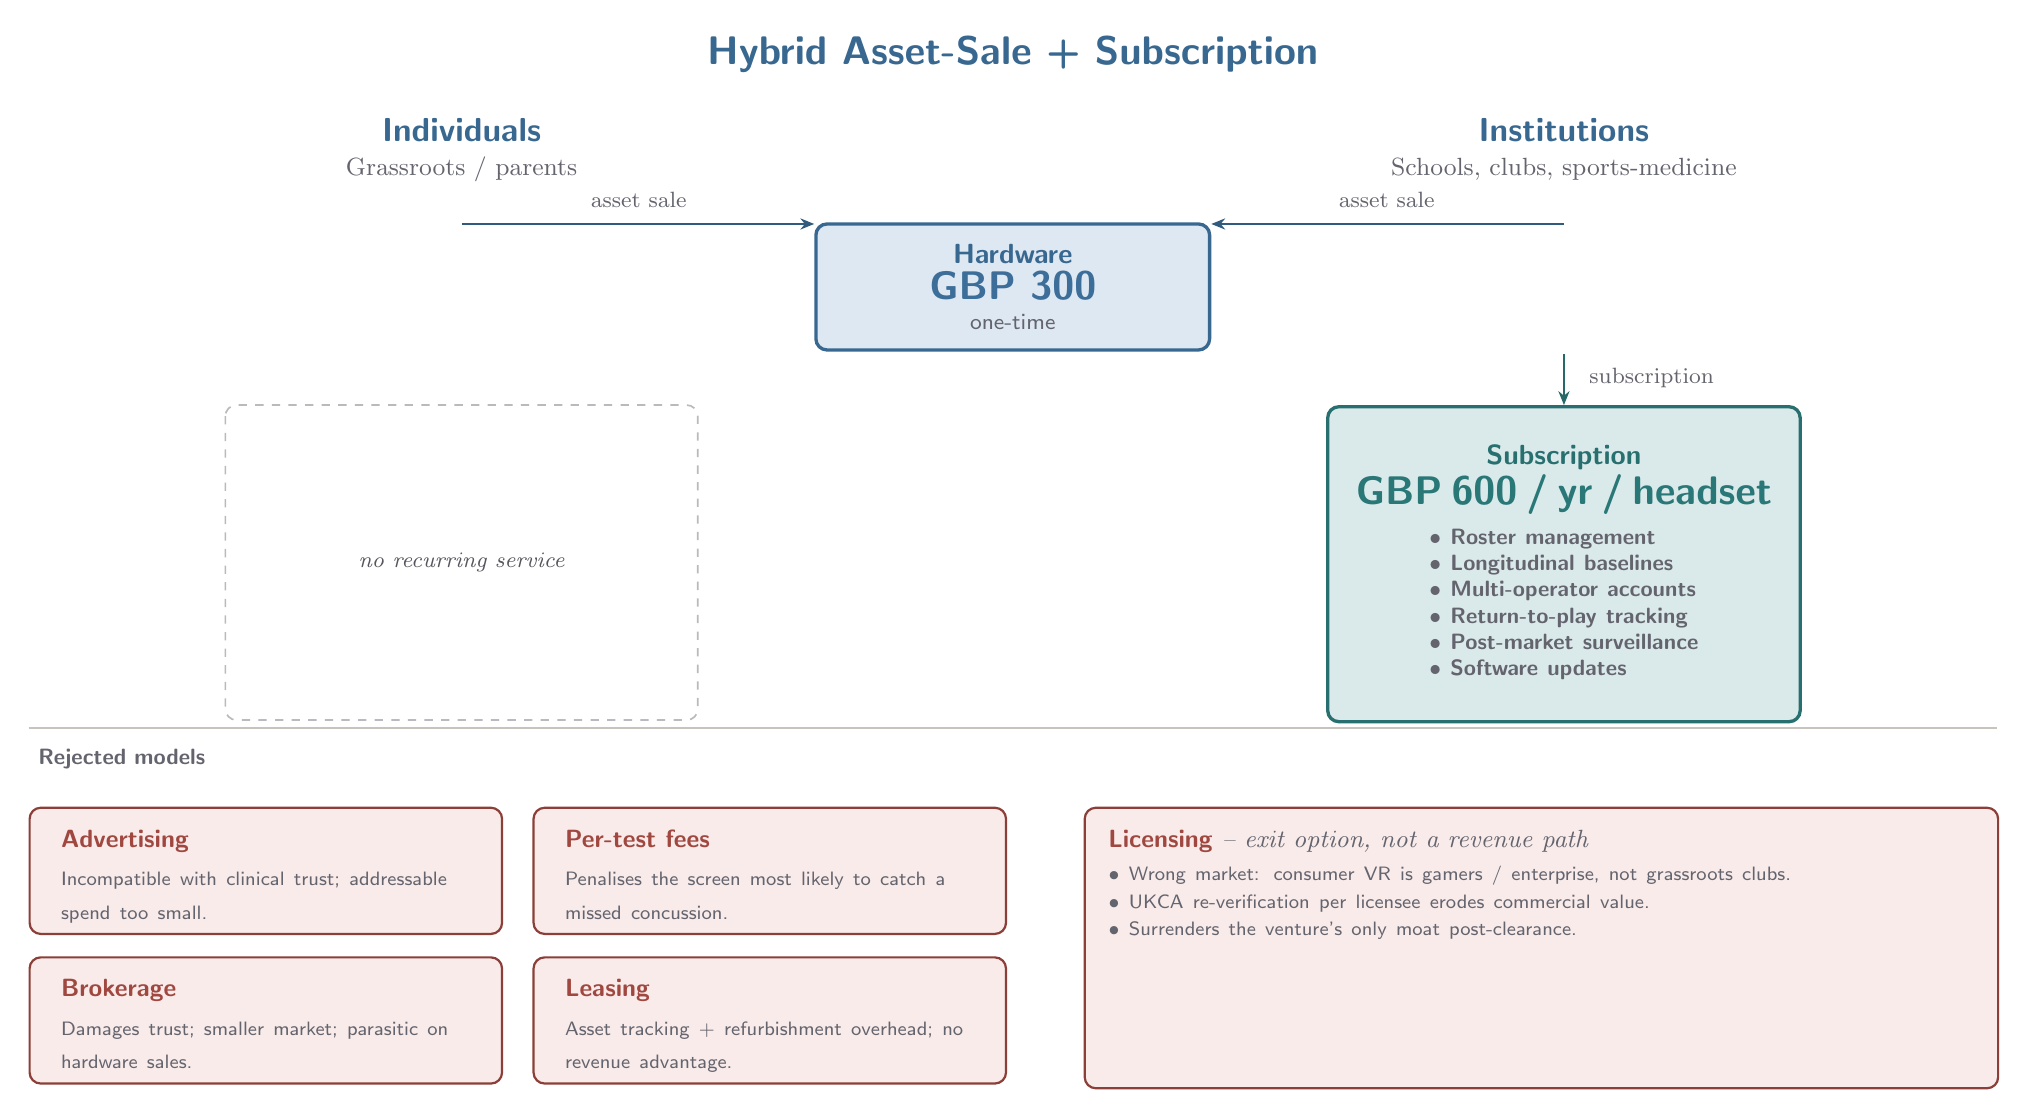
\begin{tikzpicture}[
    every node/.style={font=\sffamily},
    sel block/.style={rectangle, rounded corners=4pt, line width=1.2pt, align=center, inner sep=6pt},
    rej card/.style={rectangle, rounded corners=4pt, line width=0.8pt,
                     draw=lostred!70!black, fill=lostred!12,
                     align=left, inner sep=8pt, anchor=north west},
    arr/.style={-{Stealth[length=5pt,width=4pt]}, line width=1.0pt},
  ]

  % ============ TITLE STRIP ============
  \node[anchor=north, font=\Large\sffamily\bfseries, text=flowblue!80!black]
    at (12.5, 0.5) {Hybrid Asset-Sale + Subscription};

  % ============ BUYER COLUMN HEADERS ============
  \node[anchor=center] at (5.5, -0.8)
    {\large\sffamily\bfseries\color{flowblue!80!black}Individuals};
  \node[anchor=center, font=\small, text=neutralgrey] at (5.5, -1.3)
    {Grassroots / parents};

  \node[anchor=center] at (19.5, -0.8)
    {\large\sffamily\bfseries\color{flowblue!80!black}Institutions};
  \node[anchor=center, font=\small, text=neutralgrey] at (19.5, -1.3)
    {Schools, clubs, sports-medicine};

  % ============ HARDWARE BLOCK (centre) ============
  \node[sel block, draw=flowblue!80!black, fill=flowblue!18,
        minimum width=5cm, minimum height=1.6cm] (hw) at (12.5, -2.8) {%
    \bfseries\color{flowblue!80!black}Hardware\\[1pt]
    {\Large\bfseries\color{flowblue!85!black}GBP 300}\\[-1pt]
    {\footnotesize\color{neutralgrey}one-time}
  };

  % Arrows into hardware block (kept horizontal for clean alignment)
  \draw[arr, color=flowblue!70!black] (5.5, -2.0) -- (hw.west |- 5.5,-2.0);
  \draw[arr, color=flowblue!70!black] (19.5, -2.0) -- (hw.east |- 19.5,-2.0);

  % asset-sale labels: above the arrows, centred on each
  \node[font=\footnotesize, text=neutralgrey, anchor=south]
    at (7.75, -1.92) {asset sale};
  \node[font=\footnotesize, text=neutralgrey, anchor=south]
    at (17.25, -1.92) {asset sale};

  % ============ SUBSCRIPTION BLOCK (right only) ============
  \node[sel block, draw=solutionteal!80!black, fill=solutionteal!18,
        minimum width=6.0cm, minimum height=4.0cm,
        text width=5.4cm, anchor=north]
        (sub) at (19.5, -4.3) {%
    \bfseries\color{solutionteal!80!black}Subscription\\[1pt]
    {\Large\bfseries\color{solutionteal!85!black}GBP 600 / yr / headset}\\[3pt]
    \footnotesize\color{neutralgrey}\raggedright
    \begin{tabular}{@{}l@{}}
    $\bullet$~Roster management\\
    $\bullet$~Longitudinal baselines\\
    $\bullet$~Multi-operator accounts\\
    $\bullet$~Return-to-play tracking\\
    $\bullet$~Post-market surveillance\\
    $\bullet$~Software updates\\
    \end{tabular}
  };

  % Down-arrow Institutions -> subscription
  \draw[arr, color=solutionteal!75!black]
    (19.5, -3.65) -- (sub.north);
  \node[font=\footnotesize, text=neutralgrey, anchor=west] at (19.7, -3.95)
    {subscription};

  % ============ EMPTY-SLOT (mirrors Subscription block dimensions) ============
  % Subscription block spans x in [16.5, 22.5], y in [-4.3, -8.3]
  % Mirror under Individuals at x in [2.5, 8.5], same y range
  \draw[dashed, line width=0.6pt, color=neutralgrey!45, rounded corners=4pt]
    (2.5, -4.3) rectangle (8.5, -8.3);
  \node[anchor=center, font=\footnotesize\itshape, text=neutralgrey!85!black]
    at (5.5, -6.3) {no recurring service};

  % ============ DIVIDER ============
  \draw[linegrey, line width=0.6pt] (0, -8.4) -- (25, -8.4);
  \node[anchor=north west, font=\footnotesize\sffamily\bfseries, text=neutralgrey]
    at (0, -8.55) {Rejected models};

  % ============ REJECTED CARDS ============
  % 4 small cards in 2x2 grid, x: [0, 13]
  \def\cardW{6.0cm}
  \def\cardH{1.6cm}
  \def\cardgapX{0.4cm}
  \def\cardgapY{0.3cm}

  % Row 1
  \node[rej card, minimum width=\cardW, minimum height=\cardH, text width=5.2cm]
    at (0, -9.4) {%
      \begin{minipage}[t][1.04cm][t]{5.2cm}
      {\small\bfseries\color{lostred!80!black}Advertising}\\[2pt]
      {\scriptsize\color{neutralgrey}Incompatible with clinical trust;
      addressable spend too small.}
      \end{minipage}
    };
  \node[rej card, minimum width=\cardW, minimum height=\cardH, text width=5.2cm]
    at (6.4, -9.4) {%
      \begin{minipage}[t][1.04cm][t]{5.2cm}
      {\small\bfseries\color{lostred!80!black}Per-test fees}\\[2pt]
      {\scriptsize\color{neutralgrey}Penalises the screen most likely to catch
      a missed concussion.}
      \end{minipage}
    };

  % Row 2
  \node[rej card, minimum width=\cardW, minimum height=\cardH, text width=5.2cm]
    at (0, -11.3) {%
      \begin{minipage}[t][1.04cm][t]{5.2cm}
      {\small\bfseries\color{lostred!80!black}Brokerage}\\[2pt]
      {\scriptsize\color{neutralgrey}Damages trust; smaller market;
      parasitic on hardware sales.}
      \end{minipage}
    };
  \node[rej card, minimum width=\cardW, minimum height=\cardH, text width=5.2cm]
    at (6.4, -11.3) {%
      \begin{minipage}[t][1.04cm][t]{5.2cm}
      {\small\bfseries\color{lostred!80!black}Leasing}\\[2pt]
      {\scriptsize\color{neutralgrey}Asset tracking + refurbishment overhead;
      no revenue advantage.}
      \end{minipage}
    };

  % Wide Licensing card (right half) -- top-aligned content
  \node[rej card, minimum width=11.6cm, minimum height=3.5cm, text width=11.0cm,
        inner sep=8pt]
    at (13.4, -9.4) {%
      \begin{minipage}[t][3.0cm][t]{11.0cm}%
      {\small\bfseries\color{lostred!80!black}Licensing
      \normalfont\itshape\color{neutralgrey} -- exit option, not a revenue path}\\[4pt]
      \scriptsize\color{neutralgrey}\raggedright
      $\bullet$~Wrong market: consumer VR is gamers / enterprise, not grassroots clubs.\\[2pt]
      $\bullet$~UKCA re-verification per licensee erodes commercial value.\\[2pt]
      $\bullet$~Surrenders the venture's only moat post-clearance.
      \end{minipage}
    };

\end{tikzpicture}
\end{document}
